\documentclass{article}

% if you need to pass options to natbib, use, e.g.:
% \PassOptionsToPackage{numbers, compress}{natbib}
% before loading neurips_2024

% \usepackage{neurips_2024}        % for submission
\usepackage[final]{neurips_2024}   % for camera-ready version

\usepackage[utf8]{inputenc} % allow utf-8 input
\usepackage[T1]{fontenc}    % use 8-bit T1 fonts
\usepackage{hyperref}       % hyperlinks
\usepackage{url}            % simple URL typesetting
\usepackage{booktabs}       % professional-quality tables
\usepackage{amsfonts}       % blackboard math symbols
\usepackage{nicefrac}       % compact symbols for 1/2, etc.
\usepackage{microtype}      % microtypography
\usepackage{xcolor}         % colors
\usepackage{graphicx}
\usepackage{amsmath}
\usepackage{amssymb}
\usepackage{caption}
\usepackage{subcaption}
\usepackage{float}

\graphicspath{ {./images/} }

\title{Multimodal Deep Learning for Single-Cell Analysis}

\author{%
  Denis Grachev \\
  TUM \\
  \texttt{justwantpost@gmail.com} \\
}

\begin{document}

\maketitle

\begin{abstract}
Single-cell analysis has revolutionized our understanding of cellular heterogeneity, 
providing a high-resolution view of molecular features (e.g., transcriptomics, proteomics) 
in individual cells. However, analyzing multiple modalities simultaneously can be complex 
due to high dimensionality, sparsity, and batch effects. In this report, we apply 
multimodal deep learning to single-cell data integration, focusing on models like 
Multigrate, TOTALVI, and MOFA. Each model produces low-dimensional embeddings for every cell, 
which are then converted into a cell-cell graph. We evaluate the quality of these embeddings 
via graph-based metrics such as ARI, NMI, Silhouette Score, Graph Connectivity, 
and Isolated Labels ASW. Our findings highlight the promise of deep learning in capturing 
the interrelationships among diverse molecular measurements.
\end{abstract}

\section{Introduction}
Single-cell technologies capture gene expression, chromatin accessibility, or protein abundance 
at single-cell resolution, providing unprecedented insight into cellular heterogeneity. 
Yet these data come from different modalities, so integrative methods are needed to combine 
genomics, transcriptomics, proteomics, and other assays. Deep learning approaches 
offer flexible frameworks for learning shared representations of multimodal data, 
while also helping to mitigate common challenges like batch effects.

In this report, we examine a benchmark multimodal single-cell dataset, describe 
a preprocessing pipeline, and present three representative models---Multigrate, TOTALVI, and MOFA---for integrated analysis. 
After each model learns embeddings for the cells, we build a cell-cell graph 
to compute a variety of metrics (e.g., ARI, NMI). We compare the models’ performance 
and discuss the trade-offs involved in single-cell data integration.

\section{Data}
The dataset used in this study comprises approximately 120,000 human bone marrow cells 
collected from 10 donors. Measurements come from two main assay combinations: 
(1) nuclear gene expression (GEX) plus ATAC, and (2) cellular GEX plus antibody-derived tags (ADT). 
Nested batch effects are introduced by sampling each donor at four different laboratory sites, 
thus representing both site- and donor-level variability. Each cell contains:
\begin{itemize}
    \item \textbf{ATAC}: Accessibility of 119,254 genomic regions.
    \item \textbf{GEX}: Expression levels of 15,189 genes.
    \item \textbf{ADT}: Abundance of 134 surface proteins.
\end{itemize}

The dataset covers multiple developmental lineages, including immune populations 
and erythrocyte precursors. Data preprocessing and annotation were performed 
using standardized pipelines with quality control, normalization, clustering, 
and trajectory inference. Ground-truth cell identities were assigned 
through expert curation and marker-based annotation.

\begin{figure}[H]
  \centering
  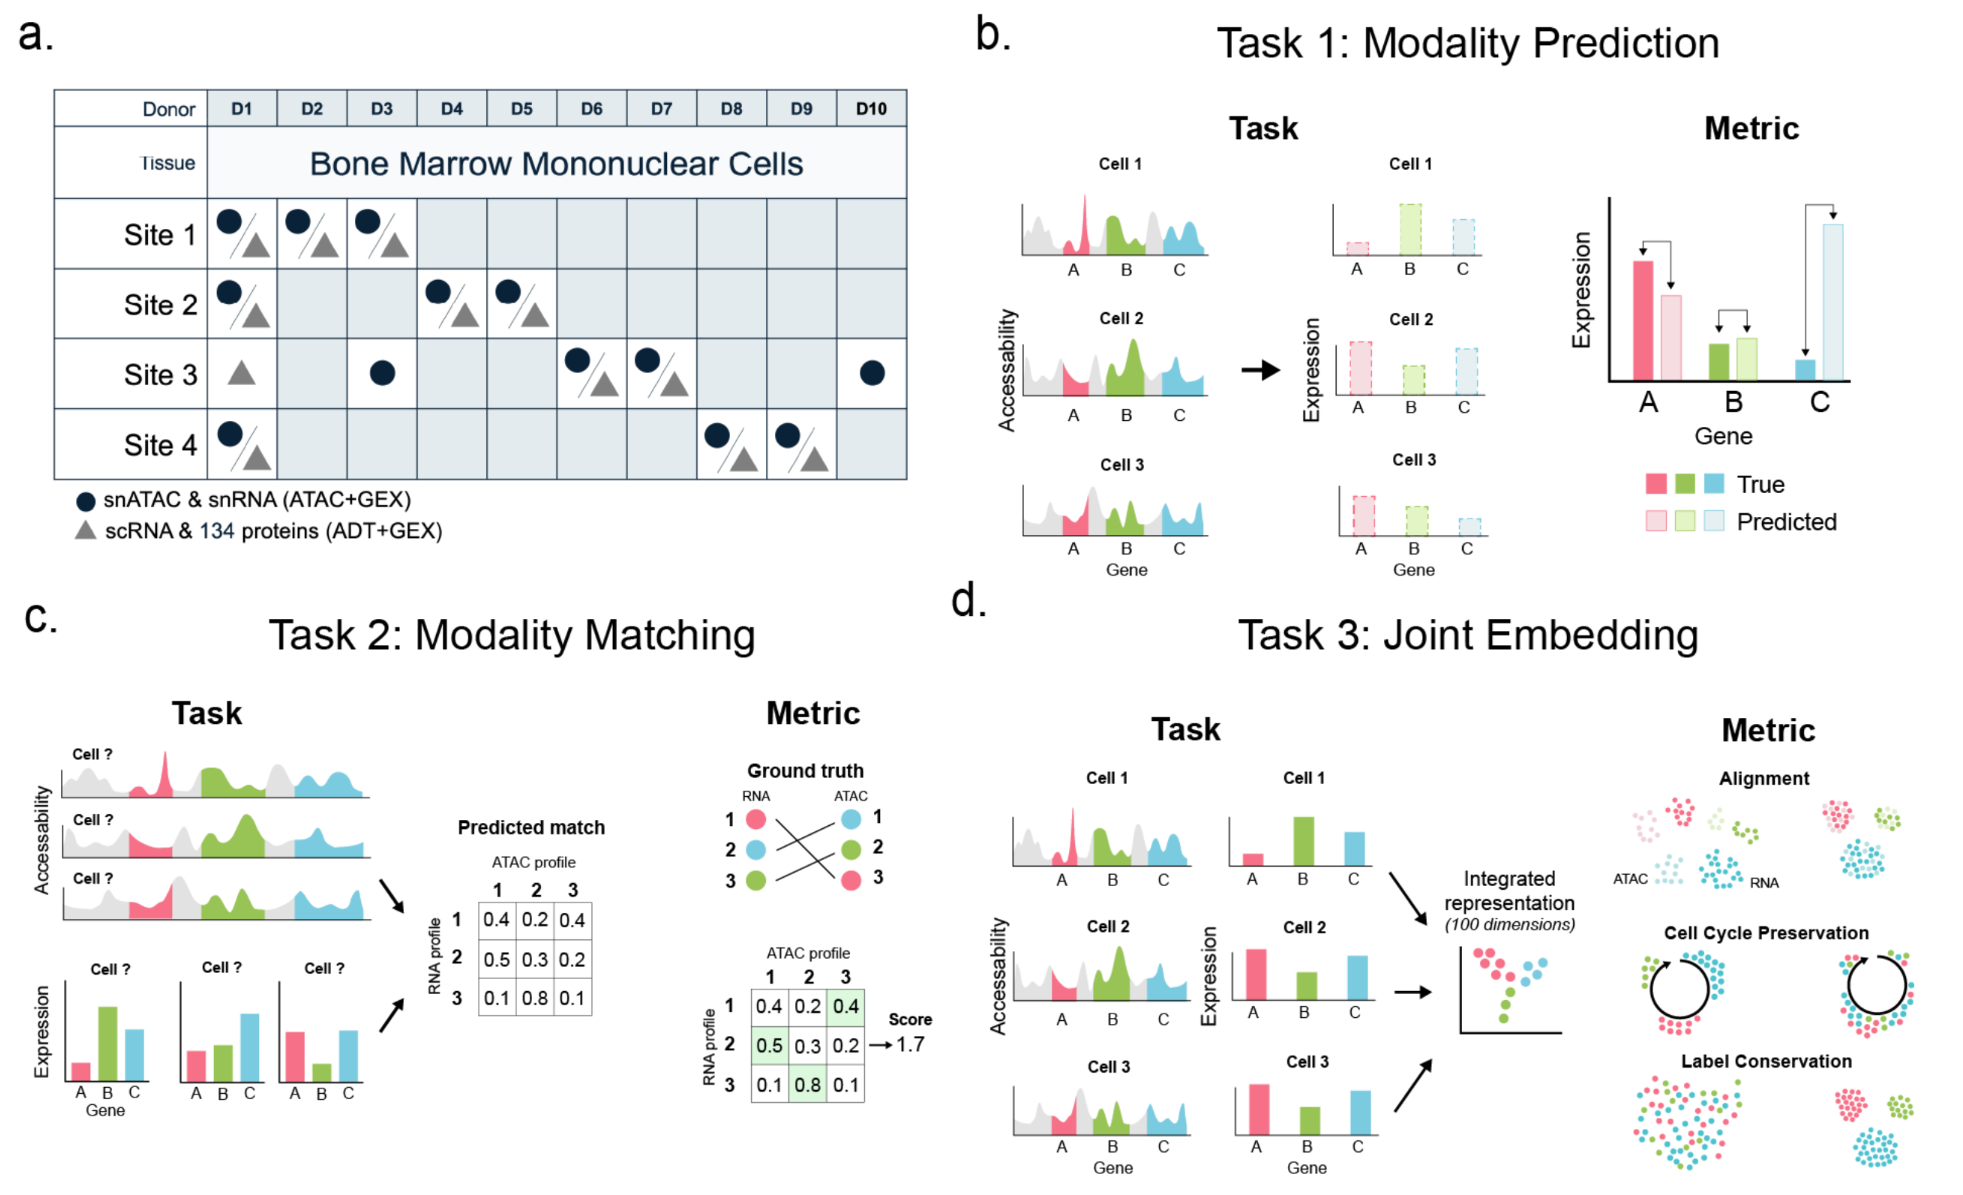
\includegraphics[width=0.8\linewidth]{multimodal_intro}
  \caption{ Overview of a multimodal single-cell reference dataset and the three principal tasks: 
  (a) multi-site BMMC data with known annotations, 
  (b-d) modality prediction, matching, and joint representation \cite{luecken2020sandbox}.}
  \label{fig:dataset}
\end{figure}

\section{Data Preprocessing}
Before training the models, we perform essential preprocessing steps to ensure consistent 
and comparable inputs across different modalities:

\begin{enumerate}
    \item \textbf{Subsampling}: For demonstration or memory considerations, the data may be subsampled 
    (e.g., to 20,000 cells) to reduce computational load. Subsampling allows rapid prototyping 
    without qualitatively changing core results, especially when dealing with very large datasets.
    \item \textbf{Splitting RNA and ADT}: The GEX features are extracted as an \(\texttt{AnnData}\) object (\texttt{rna}), 
    while the ADT features are kept in a separate \(\texttt{AnnData}\) (\texttt{adt}). 
    This separation is convenient for multi-omics pipelines (e.g., MuData structures).
    \item \textbf{Layer Allocation}: For RNA, we copy \(\texttt{layers["counts"]}\) into \(\texttt{.X}\) so that normalization 
    is based on raw counts. This ensures that the standard single-cell protocols (e.g., \texttt{sc.pp.normalize\_total}, \texttt{sc.pp.log1p}) are applied consistently.
    \item \textbf{Normalization and Log-Transform} (RNA): 
    Total count normalization (target sum \(= 10^4\)) followed by a log(1 + \(\cdot\)) transform 
    to stabilize variance and reduce skew.
    \item \textbf{Highly Variable Gene (HVG) Selection}: 
    We identify the top 2,000 HVGs, considering \(\texttt{Site}\) as a batch variable to adjust for batch-specific differences. 
    Retaining only HVGs can improve downstream model performance by focusing on the most informative transcripts.
    \item \textbf{CLR Transform (ADT)}: For the ADT features, a centered log-ratio (\texttt{clr}) normalization 
    is often recommended, as it helps control for differences in overall protein capture efficiency. 
    The \(\texttt{muon.prot.pp.clr}\) function performs this step, storing the result in \(\texttt{.X}\).
    \item \textbf{MuData Assembly}: We can merge the preprocessed \texttt{rna} and \texttt{adt} \(\texttt{AnnData}\) objects 
    into a single \(\texttt{MuData}\) container (\(\texttt{mdata}\)), preserving separate modalities but allowing integrated analysis.
\end{enumerate}

After these steps, the dataset is better suited for models that integrate multiple omics layers, 
each modality having been normalized and transformed appropriately for the model’s assumptions.

\section{Batch Effect Correction}
Single-cell data can exhibit significant batch effects due to technical or procedural variation. 
If not corrected, these effects may obscure true biological signals. Common strategies include:

\begin{itemize}
 \item \textbf{Linear Methods (e.g., ComBat, limma)}:  
   Model batch as an additive or multiplicative term in a linear framework.
 \item \textbf{Nonlinear Methods (e.g., MNN, CCA)}:  
   Align data through mutual nearest neighbors or canonical correlations to capture complex batch effects.
 \item \textbf{Deep Learning Methods (e.g., VAEs)}:  
   Learn latent spaces where batch variation is separated from biological signals.
\end{itemize}

\begin{figure}[H]
  \centering
  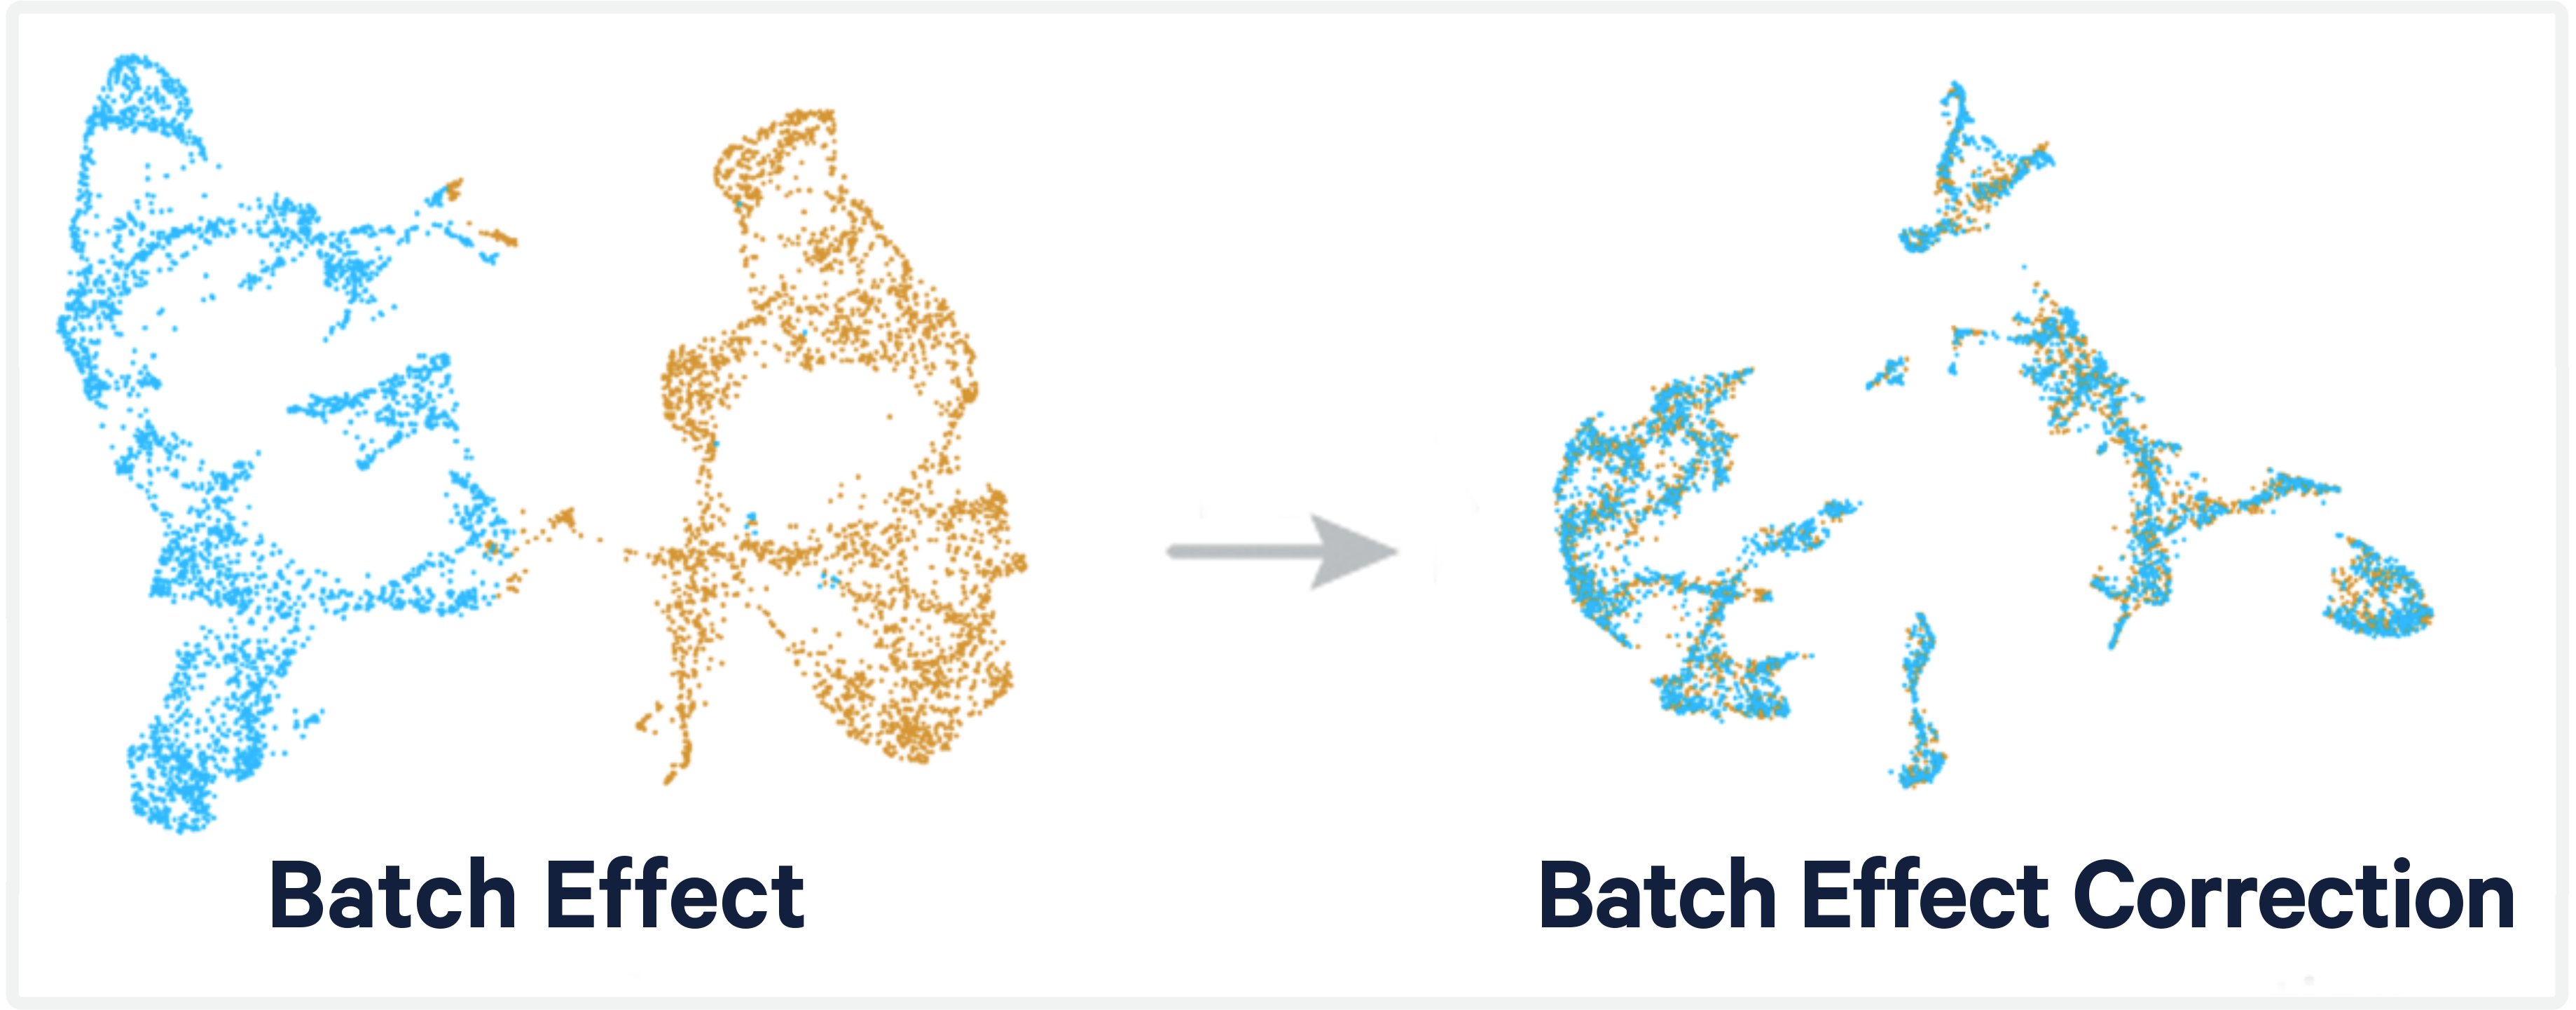
\includegraphics[width=0.8\linewidth]{BatchCorrection}
  \caption{Diagram of batch effect (left) and corrected data (right) \cite{10xgenomics_batch_effect}.}
  \label{fig:batch_effect}
\end{figure}

\section{Models}
We apply three models designed for multimodal single-cell data. Each model outputs a latent embedding 
for each cell. We then construct a \emph{cell-cell graph} (e.g., using \(k\)-nearest neighbors) 
based on these embeddings, which forms the basis of the evaluation metrics.

\subsection{Multigrate Architecture}
\label{sec:multigrate}
Multigrate is a generative multi-view neural network capable of handling missing modalities 
and batch covariates \cite{lotfollahi2022multigrate}. It adopts a Product of Experts (PoE) approach 
to fuse the latent representations of different data types.

\begin{figure}[H]
  \centering
  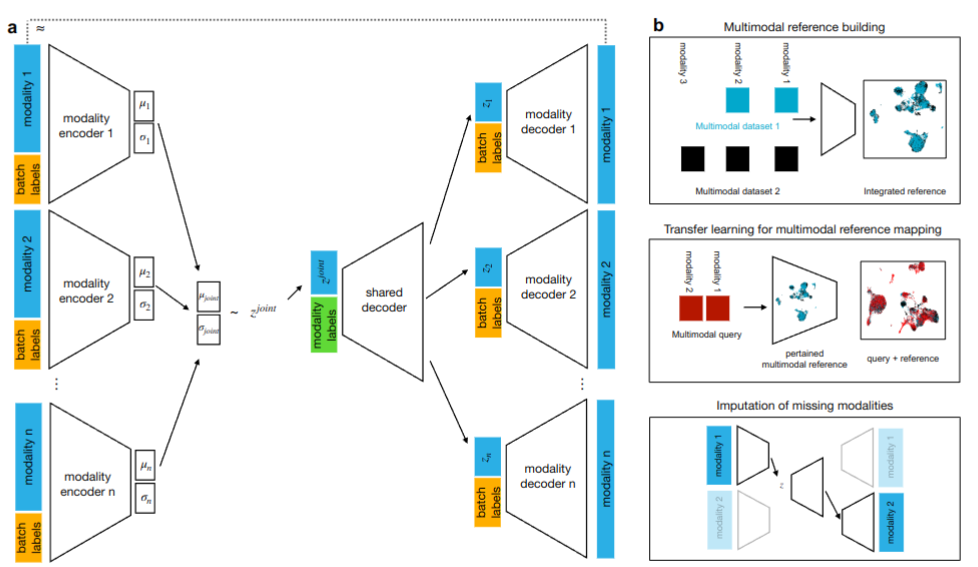
\includegraphics[width=0.8\linewidth]{multigrate_architecture}
  \caption{Multigrate architecture \cite{lotfollahi2022multigrate}.}
  \label{fig:multigrate_architecture}
\end{figure}

\subsubsection{Generative Model}
Let \(X = \{ X_i \}_{i=1}^{n}\) be observations from \(n\) modalities, 
and \(S = \{ S_i \}_{i=1}^{n}\) be study labels encoding batch/site. 
When a modality \(i\) is absent, the corresponding \(X_i\) is empty.

Using PoE, the approximate posterior is:
\begin{equation}
    q_{\phi}(Z_{\text{joint}} \mid X, S) = \prod_{i=1}^{n} q_{\phi_i}(Z_i \mid X_i, S_i),
\end{equation}
where \(q_{\phi_i}(Z_i \mid X_i, S_i)=1\) if modality \(i\) is missing, 
otherwise it is a Gaussian \(\mathcal{N}(\mu_i, \sigma_i)\). 
The joint distribution is computed via:
\begin{align}
    \mu_{\text{joint}} &= \left(\mu_0 \sigma_0^{-1} + \sum_{i=1}^{n} m_i \mu_i \sigma_i^{-1} \right)
                         \left( \sigma_0^{-1} + \sum_{i=1}^{n} m_i \sigma_i^{-1} \right)^{-1}, \\
    \sigma_{\text{joint}} &= \Bigl(\sigma_0^{-1} + \sum_{i=1}^{n} m_i \sigma_i^{-1}\Bigr)^{-1},
\end{align}
where \(m_i=1\) if modality \(i\) is present, and \(\mu_0, \sigma_0\) are prior parameters.

\subsubsection{Training Objective}
The model minimizes:
\begin{equation}
    L_{AE} = \alpha \,\mathbb{E}_{q_{\phi}(Z_{\text{joint}} \mid X_i, S_i)}\bigl[\log p_{\theta}(X_i \mid Z_{\text{joint}}, S_i)\bigr]
    - \eta \,D_{\mathrm{KL}}\bigl(q_{\phi}(Z_{\text{joint}} \mid X_i, S_i)\,\|\, p_{\theta}(Z_{\text{joint}} \mid S_i)\bigr),
\end{equation}
summed over all modalities. An MMD term aligns latent spaces across batches:
\[
L_{\mathrm{MMD}}(Z_{\text{joint}_i}, Z_{\text{joint}_j}) 
= \sum_{i<j} k(Z_{\text{joint}_i},\, Z_{\text{joint}_j}, \gamma),
\]
where \(k\) is a multi-scale RBF kernel. The total loss is:
\begin{equation}
    L_{\mathrm{Multigrate}} = \sum_{i=1}^{n} L_{AE}(X_i, S_i) + \beta \sum_{i<j} L_{\mathrm{MMD}}(Z_{\text{joint}_i}, Z_{\text{joint}_j}).
\end{equation}

\subsection{TOTALVI Architecture}
\label{sec:totalvi}
TOTALVI is a deep generative model for jointly analyzing RNA and protein data \cite{gayoso2021joint}. 
It uses a VAE-like framework that accounts for batch effects and protein background noise.

\subsubsection{Generative Model}
Each cell \(n\) has:
\[
x_n \in \mathbb{R}^{G} \quad(\text{RNA counts}), \quad
y_n \in \mathbb{R}^{T} \quad(\text{protein counts}),
\]
and a one-hot batch vector \(s_n\). The latent variable \(z_n\) follows a LogisticNormal prior, 
while \(\ell_n\) accounts for RNA library size.

RNA counts follow a Gamma-Poisson mixture:
\[
x_{ng} \mid z_n, \ell_n \,\sim\, \text{NegativeBinomial}(\ell_n \,\rho_{ng}, \,\theta_g),
\]
and proteins use a mixture distribution that handles background:
\[
y_{nt} \mid z_n \,\sim\, \text{Poisson}(r_{nt}), 
\]
where \(r_{nt}\) depends on latent variables for protein expression and background.

\subsubsection{Inference Model}
Approximate posteriors:
\[
q_{\phi}(z_n \mid x_n, y_n, s_n), \quad
q_{\phi}(\ell_n \mid x_n, s_n), \quad
q_{\phi}(\pi_{nt} \mid y_n), 
\]
are parameterized by neural networks.

\subsubsection{Optimization}
TOTALVI maximizes the ELBO:
\[
\mathcal{L}_{\mathrm{TOTALVI}}
= \mathbb{E}_{q_{\phi}(z_n \mid x_n, y_n, s_n)} \bigl[\log p_{\theta}(x_n, y_n \mid z_n, s_n)\bigr]
- D_{\mathrm{KL}}\bigl(q_{\phi}(z_n \mid x_n, y_n, s_n)\,\|\,p(z_n)\bigr).
\]
This yields latent embeddings correcting for batch and separating background signals from true protein counts.

\subsection{MOFA Architecture}
\label{sec:mofa}
Multi-Omics Factor Analysis (MOFA) factorizes multi-view data into shared latent factors \cite{https://doi.org/10.15252/msb.20178124}. 
Each modality \(m\) is expressed as:
\[
Y_m = Z W_m^T + \epsilon_m,
\]
where \(Z\in\mathbb{R}^{N\times K}\) is a latent factor matrix, 
\(W_m\in\mathbb{R}^{D_m\times K}\) are modality-specific loadings, and \(\epsilon_m\) is noise. 
Different likelihoods (Gaussian, Poisson, Bernoulli) accommodate diverse data types.

An ARD prior encourages sparsity:
\[
W_{mkd} = s_{mkd}\,\tilde{W}_{mkd}, \quad s_{mkd}\sim \mathrm{Bernoulli}(h_{mk}), 
\]
and inference uses a variational approach:
\[
q(Z,W) \approx p(Z, W \mid Y),
\]
maximizing the ELBO
\[
\mathcal{L}_{\mathrm{MOFA}} = \mathbb{E}_{q(Z,W)}[\log p(Y\mid Z,W)] - D_{\mathrm{KL}}(q(Z,W)\,\|\,p(Z,W)).
\]

\section{Metrics}
Once a model provides a latent embedding for each cell, we construct a graph (e.g., \(k\)-nearest neighbors) 
and evaluate the following:

\subsection{Adjusted Rand Index (ARI)}
Compares cluster assignments (from either known labels or graph-based partitions) to the embedding-based clustering, 
adjusted for random chance.

\subsection{Normalized Mutual Information (NMI)}
Measures information overlap between inferred clusters and known labels, normalized to lie between 0 and 1.

\subsection{Silhouette Score}
A distance-based measure of cluster separation. For each cell \(i\), let \(a(i)\) be the average distance 
to neighbors in the same cluster, and \(b(i)\) the average distance to the nearest different cluster:
\[
s(i) = \frac{b(i) - a(i)}{\max(a(i), b(i))}.
\]

\subsection{Graph Connectivity}
Examines the connectivity of the cell-cell graph itself, for instance via average shortest path length 
or the fraction of cells in the main connected component.

\subsection{Isolated Labels ASW}
Focuses on the silhouette width of rare or isolated cell types, capturing whether minority populations 
are well-separated in the embedding.

\section{Results}
We trained the three models (MOFA, TOTALVI, and Multigrate) on the processed dataset, 
obtained latent embeddings, and built a \(k\)-nearest-neighbors graph in each embedding space. 
Table~\ref{tab:results} compares ARI, NMI, Silhouette Score, Graph Connectivity, 
and Isolated Labels ASW across models.

\begin{table}[H]
\centering
\begin{tabular}{lccc}
\toprule
\textbf{Metric} & \textbf{MOFA} & \textbf{TOTALVI} & \textbf{Multigrate} \\
\midrule
ARI                   & 0.50 & 0.69 & \textbf{0.73} \\
NMI                   & 0.64 & \textbf{0.79} & 0.77 \\
Silhouette Score      & 0.54 & 0.55 & \textbf{0.59} \\
Graph Connectivity    & 0.79 & \textbf{0.91} & 0.88 \\
Isolated Labels ASW   & \textbf{0.63} & 0.59 & 0.60 \\
\bottomrule
\end{tabular}
\caption{Performance of each model, computed on a cell-cell graph built from the learned embeddings.}
\label{tab:results}
\end{table}


TOTALVI yields the highest NMI and Graph Connectivity, reflecting well-preserved local and global structure. 
Multigrate slightly outperforms the others on ARI, indicating strong alignment with known labels. 
MOFA shows competitive performance overall, especially for isolated cell populations (higher ASW). 

\section{Conclusion}
In this report, we explored how multimodal deep learning approaches can integrate single-cell assays, 
ranging from gene expression to surface protein abundance. We introduced a benchmark multimodal dataset, 
performed a standard preprocessing pipeline (subsampling, normalization, HVG selection, CLR transform), 
and compared three models: Multigrate, TOTALVI, and MOFA. Each model provides a latent embedding 
that we transform into a cell-cell graph for computing metrics such as ARI, NMI, Silhouette Score, 
Graph Connectivity, and Isolated Labels ASW.

Our results illustrate how different model architectures excel in distinct metrics. For instance, 
TOTALVI appears to maintain high connectivity and robust gene-protein integration, while Multigrate 
performs especially well in aligning latent clusters to known cell annotations (high ARI). 
MOFA, in turn, excels at resolving certain smaller cell subsets. Overall, multimodal deep learning 
continues to advance our ability to decode complex cell heterogeneity by leveraging multiple types of 
molecular measurements within a unified framework.
\begin{figure}[h]
    \centering
    %-- Subfigure 1
    \begin{subfigure}{0.8\linewidth}
        \centering
        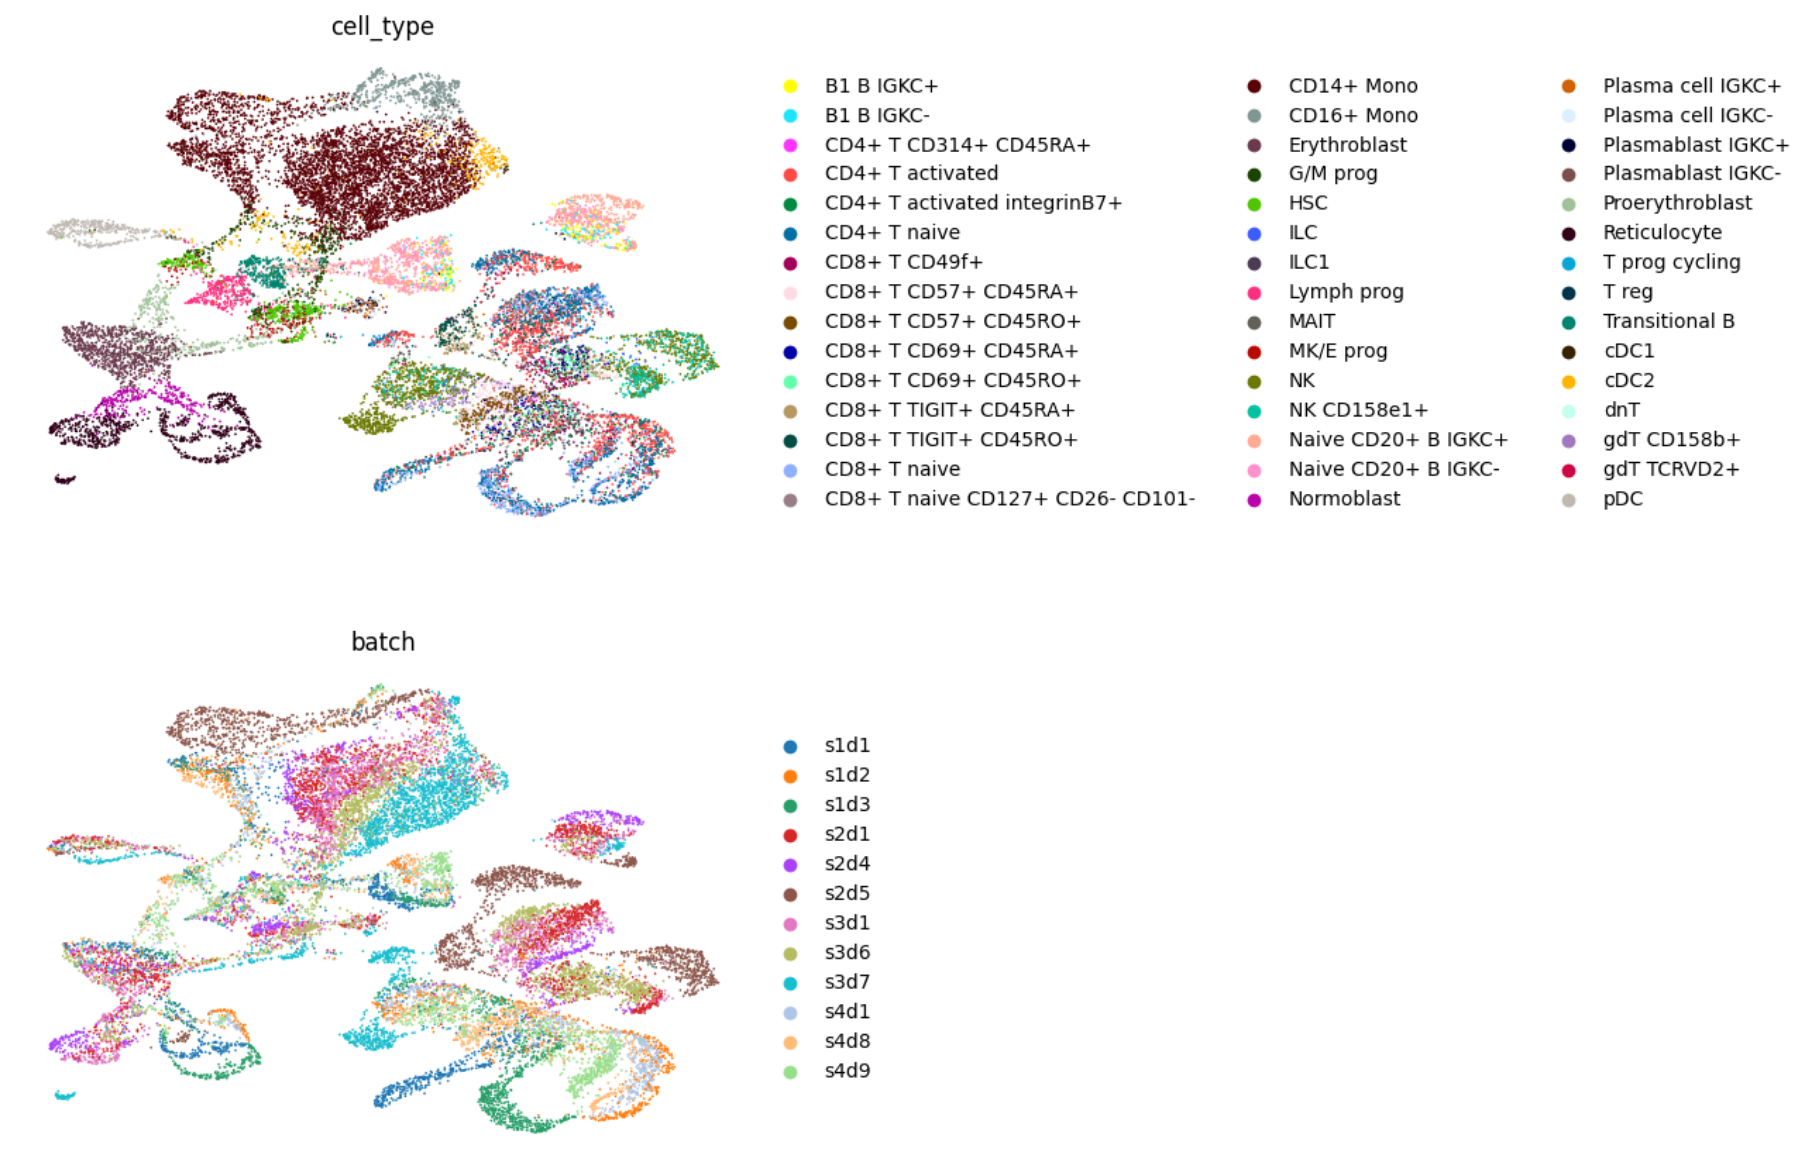
\includegraphics[width=\linewidth]{mofa_integration}
        \caption{MOFA UMAP}
        \label{fig:mofaintegration}
    \end{subfigure}
    
    \vspace{1em}
    %-- Subfigure 2
    \begin{subfigure}{0.8\linewidth}
        \centering
        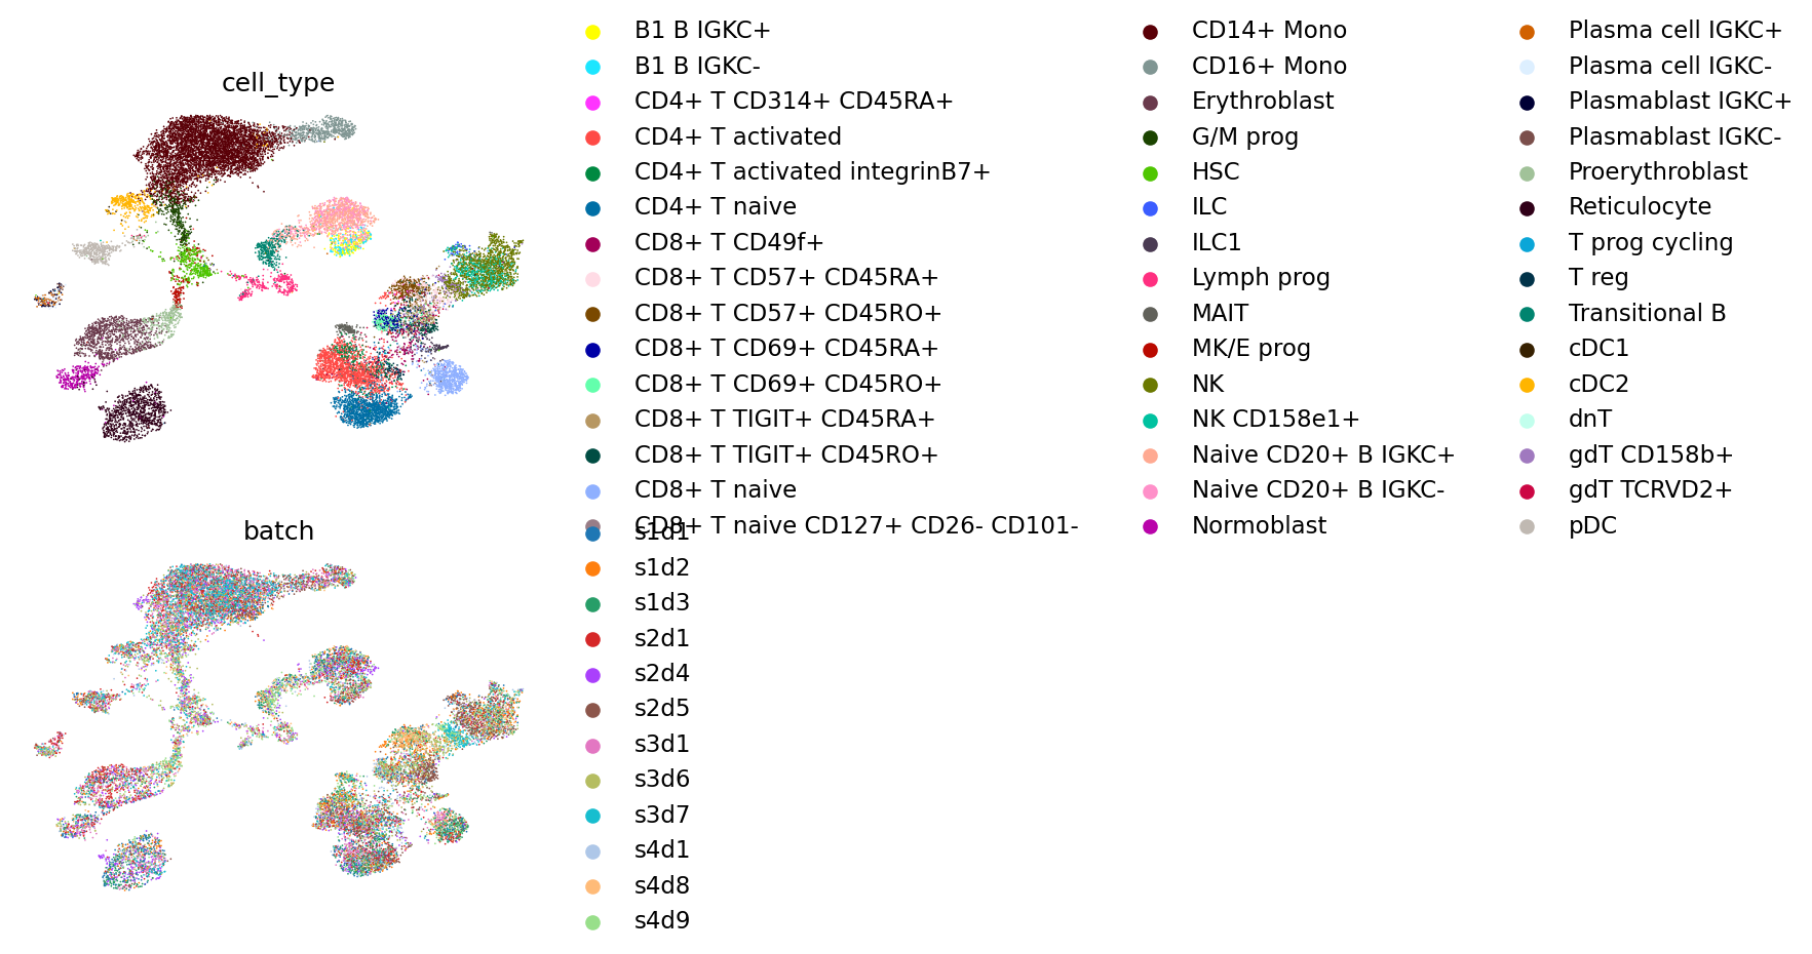
\includegraphics[width=\linewidth]{totalvi_integration}
        \caption{TOTALVI UMAP}
        \label{fig:totalviintegration}
    \end{subfigure}
    
    \vspace{1em}
    %-- Subfigure 3
    \begin{subfigure}{0.8\linewidth}
        \centering
        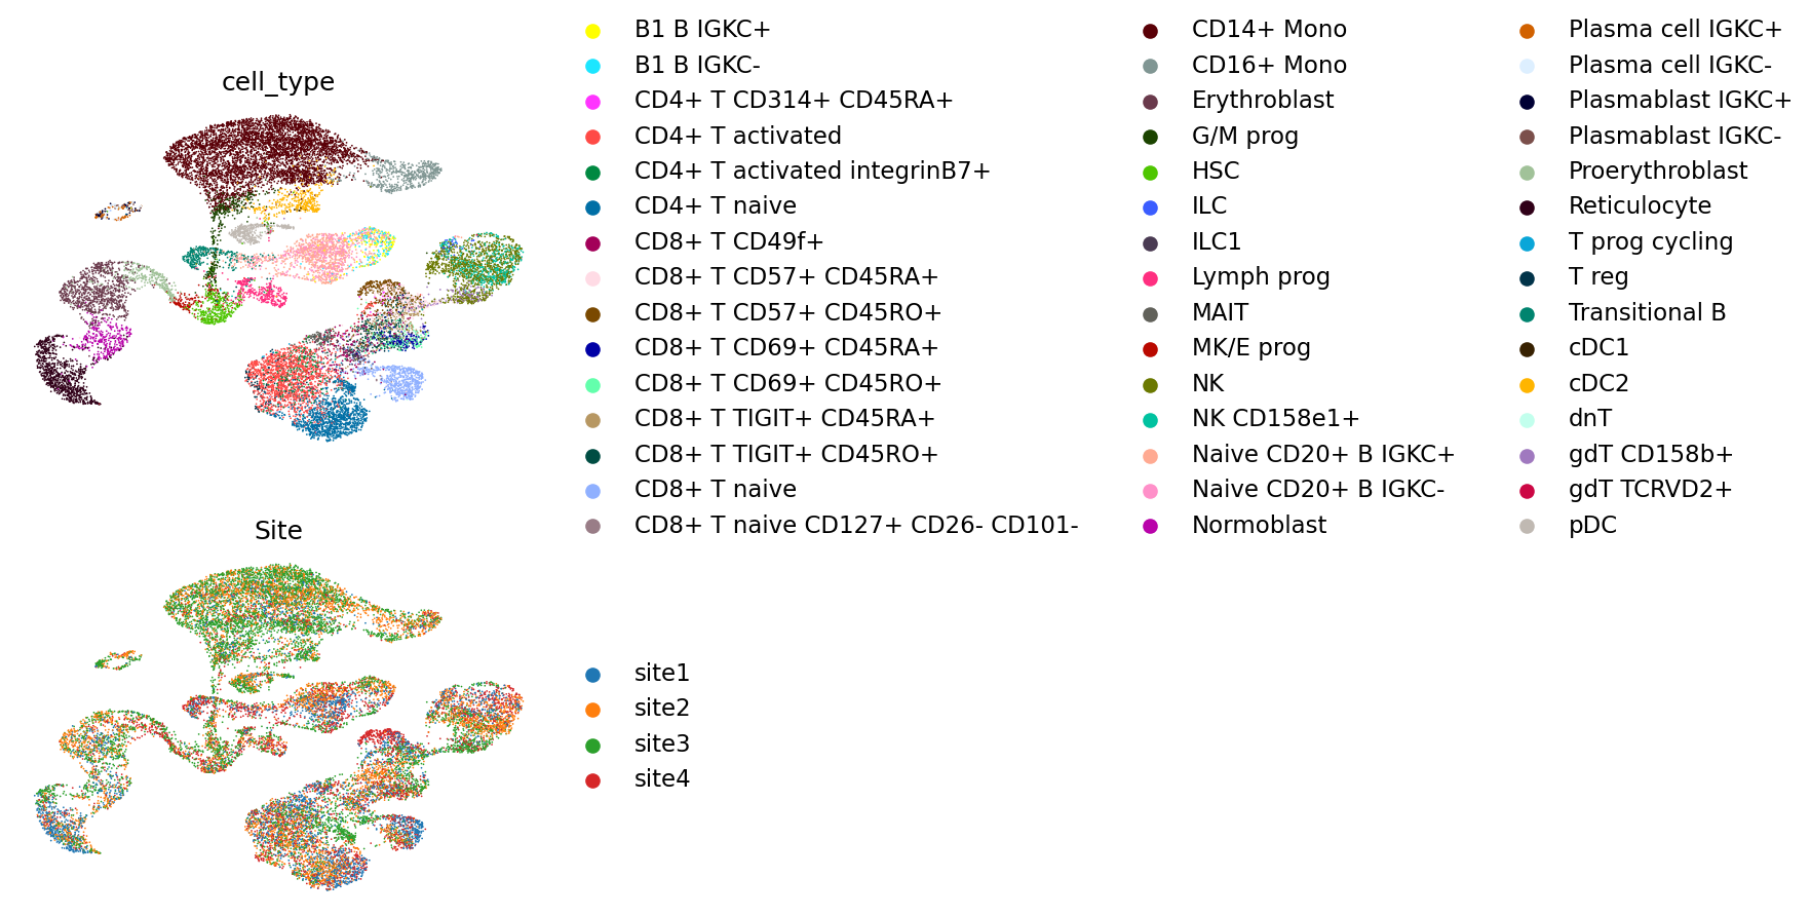
\includegraphics[width=\linewidth]{multigrate_integration}
        \caption{Multigrate UMAP}
        \label{fig:multigrateintegration}
    \end{subfigure}
    \caption{UMAP projections of the latent embeddings for (a) MOFA, (b) TOTALVI, and (c) Multigrate. 
    Here, each plot is stacked vertically rather than side by side.}
\end{figure}
\bibliography{refs}
\bibliographystyle{plain}

\end{document}
